\chapter{光场的动力学方程}
\label{chap:model1}

\fontsize{12bp}{14.4pt}

\section{泵浦-增益-激射}
三能级系统中,当上中能级之间的跃迁速率远快于中下时,给予下上能级间的泵浦即可在中下之间形成粒子数反转。\\
泵浦光被消耗,将处于低能级的Er离子泵到高能级上,再迅速落入中间能级。
信号光从初始噪声中长出,消耗反转粒子数,以平衡损耗。\\
\subsection{增益介质的方程}
设三个能级上的粒子数从低能级到高能级依次为:$N_1, N_2, N_3$。\\
粒子数守恒:
\[N = N_1 + N_2 + N_3\]
三个能级间两两可以跃迁,共有三个过程。其中下能级到上能级对应泵浦光$1480nm$;
中间能级到下能级对应信号光$1530nm$;上能级到中间能级为无辐射跃迁。\\
\[\frac{dN_1}{dt} = -R_p^a N_2 + R_p^e N_3 - R_s^a N_1 + R_s^e N_2 + \frac{1}{\tau_g} N_2\]
\[\frac{dN_2}{dt} = -R_s^e N_2 + R_s^a N_1 - \frac{1}{\tau_g} N_2 + \gamma_{23} N_3\]
\[\frac{dN_3}{dt} = R_p^a N_1 - R_p^e N_3 - \gamma_{23} N_3\]
其中,$R_{p,s}^{a,e}$为各跃迁过程的速率,与增益介质的散射截面相关:
\[R_{p,s}^{a,e} = \frac{\sigma_{p,s}^{a,e} \Gamma_{p,s}}{h\nu_{p,s} A} P_{p,s}\]
无辐射跃迁的弛豫时间短,因此中间能级和上能级之间始终满足玻尔兹曼分布:
\[\beta = \frac{N_3}{N_2} = \exp{(-\frac{\Delta E}{k_B T})}\]
利用粒子数守恒和上中能级间的关系,可以用$N,N_1$表示粒子数。
\[N_2 = \frac{1 - N_1/N}{1+\beta} N,\ N_3 = \frac{\beta(1 - N_1/N)}{1+\beta} N\]
因此,三个能级的速率方程只剩下一个有效,不妨选用$N_1$:
\[\frac{dN_1}{dt} = -\frac{1}{\tau_{N_1}} (N_1 - N_{eq})\]
\subsection{光场的方程}
腔中前后两个方向的传播模式没有区别,必须同时考虑。\\
光受到的增益为:
\[\frac{d P_{p,s}^{\pm}}{dz} = \pm \Gamma_{p,s} (\sigma_{p,s}^e N_{3,2} - \sigma_{p,s}^a N_1) P_{p,s}^{\pm} \mp \alpha_0 P_{p,s}^{\pm}\]
其中$\alpha_0$为传输损耗
设信号光电场的增益为$g$,小信号增益为$g_0$:
\[g = \frac{1}{2} \Gamma_s L_d (\sigma_s^eN_2 - \sigma_s^a N_1)\]
平衡态的增益应当具有饱和的形式,而非平衡时则会弛豫到平衡,因此猜测增益的演化方程为:
\[\tau^\prime \frac{dg}{dt} = g_0 - (1+\frac{P_s}{P_{sat}}) g\]
带入之前的方程组可得:
\[\frac{1}{\tau^\prime} = \frac{1}{1+\beta} [\frac{1}{\tau_g} + (1+\beta+\beta \frac{\sigma_p^e}{\sigma_p^a})R_p^a]\]
\[P_{sat} = \frac{h \nu_s A}{\Gamma_s \tau^\prime (\sigma_s^a + \frac{1}{1+\beta}\sigma_s^e)}\]
\[g_0 = \frac{1}{2} \Gamma_s L_d \sigma_s^e N \frac{\tau^\prime}{1 + \beta} [(1 - \frac{\sigma_s^a}{\sigma_s^e} \frac{\sigma_p^e}{\sigma_p^a} \beta) R_p^a - \frac{\sigma_s^a}{\sigma_s^e} \frac{1}{\tau_g}]\]
$R_p^a$正比于泵浦光功率,因此平衡速率、信号光饱和功率正比于泵浦光功率。\\
而小信号增益$g_0$在泵浦光功率足够大时存在饱和:\\
\[g_{0,max} = \frac{1}{2} \Gamma_s L_d N \frac{\sigma_p^a \sigma_s^e - \sigma_s^a \sigma_p^e \beta}{\sigma_p^a + \beta \sigma_p^a + \beta \sigma_p^e}\]
同理可得泵浦光受到的增益:
\[g_p = \frac{1}{2} \Gamma_p L_d N \frac{\beta \sigma_p^e \sigma_s^a - \sigma_p^a \sigma_s^e}{\sigma_s^e + \sigma_s^a (1 + \beta)} + \frac{\sigma_p^e \beta + \sigma_p^a (1 + \beta)}{\sigma_s^e + \sigma_s^a (1 + \beta)} g\]
由于泵浦光波段吸收截面大于发射截面,信号光波段吸收截面小于发射截面,因此$g_p < 0$,增益介质对泵浦光实则表现为吸收。\\
\subsection{放大的自发辐射}
除了受激辐射外,增益介质中的自发辐射也被放大,表现为噪声。\\
放大自发辐射的演化方程为$~^{[7]}$:
\[\frac{d P_{ASE}}{dz} = \Gamma_s(\sigma_s^e N_2 - \sigma_s^a N_1) P_{ASE} + 2h\nu_s \Delta \nu \sigma_s^e \Gamma_s N_2 - \alpha_0 P_{ASE}\]
用只含有$g$的方程表达:
\[\frac{d P_{ASE}}{dz} = \frac{2g}{L_d} P_{ASE} + 2h\nu_s \Delta \nu \sigma_s^e \Gamma_s N_2 - \alpha_0 P_{ASE}\]
\[N_2 = \frac{N + 2g / (\Gamma_s \sigma_s^a L_d)}{1 + \beta + \sigma_s^e / \sigma_s^a}\]
带入初始值0,解得单周期ASE功率$P_{ASE0}$:
\[P_{ASE0} = h\nu_s \Delta \nu \sigma_s^e \Gamma_s N_2 L_d \frac{e^{2g} - 1}{g - l}\]
自发辐射具有相位随机性,因此单周期ASE将在加上随机相位后合并到信号光中。
\[A(0^+) = \mathcal{F}^{-1}[\mathcal{F}[A(0^-)] + \sqrt{P_{ASE}}e^{i\phi_i}]\]
\section{电光调制}
在电极上施加谐振频率的微波后,由于铌酸锂的二阶非线性效应,材料的有效折射率发生改变,相当于腔长随着时间变化,周期与脉冲周期相同。
\subsection{泵浦光--电光梳}
稳态下,泵浦光受到本征损耗和来自增益体系的稳定吸收,视作等效损耗。又受到电光调制,并且没有增益。因此泵浦光展开为电光梳。\\
电光梳的输出光场可通过简单的线性叠加获得:
\[E_{out}(t) = \sqrt{(1-\gamma)(1-k)} E_{in}(t) - k\sqrt{\frac{1-\gamma}{1-k}} \Sigma_{n=1}^{\infty}r^n e^{iMF_n(\omega_m t) E_{in}(t-nT)}\]
其中$\gamma$为输入输出耦合器插耗,$k$为其功率透过率,$r=\sqrt{\alpha(1-\gamma)(1-k)}$为单周期透过率,$1-\alpha$为单周期功率损耗比例。\\
谐振条件下:
\[F_n(\omega_m t) = \Sigma_{n=1}^{\infty} \mathrm{sin}\omega_m(t-iT)\]
\[E_{out}(t) = \sqrt{(1-\gamma)(1-k)} \hat{E_{in}}e^{i\omega_0 t} - k\sqrt{\frac{1-\gamma}{1-k}} \frac{r e^{iMsin\omega_m t}}{1-r e^{iMsin\omega_m t}} \hat{E_{in}}e^{i\omega_0 t}\]
对于泵浦光,设吸收效率为$\eta$,则有:
\[P_0 = (1-\gamma)(1-k)P_{in} |1-\frac{k}{1-k}\Sigma_{n=1}^{\infty}r^n J_0(nM)|^2\]
\[\eta = |\frac{1-k-k\Sigma_{n=1}^{\infty}r^n J_0(nM)}{1-k-k\frac{r}{1-r}}|^2\]
\begin{figure}[htbp]
    \centering
    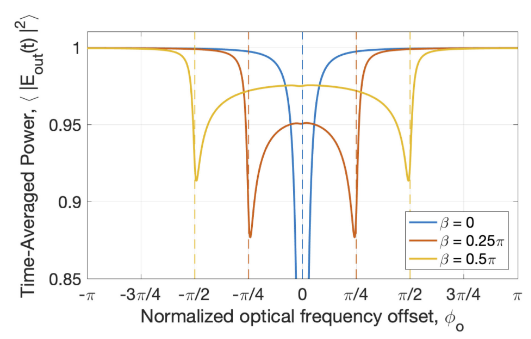
\includegraphics[width=0.8\linewidth]{figure/fig_11.png}
    \caption{不同调制深度下的谐振峰透过谱}
    \label{fig:enter-label}
\end{figure}
泵浦吸收效率$\eta$没有简约的数学表达式。
\subsection{信号光--锁模激光器}
稳态下,信号光受到本征损耗和增益,受到电光调制,形成主动锁模激光器。\\
信号光的演化由Haus方程描述:
\[T_R \frac{\partial A}{\partial T} = (-l + g(\omega) + i\delta |A|^2 - iD\frac{\partial^2}{\partial t^2} + iM\mathrm{cos}\omega_m t) A \]
有限的增益带宽:
\[g(\omega) = \frac{g}{1+(\omega - \omega_s)^2/\Omega_g^2}\]
小量近似,可将Haus方程进一步展开:
\[T_R \frac{\partial A}{\partial T} = (-l + g + i\delta |A|^2 + (iD + \frac{g}{\Omega_g^2})\frac{\partial^2}{\partial t^2} + iM(1 - \frac{1}{2} \omega_m^2 t^2))) A \]
稳态方程没有解析解,但在一定的参数条件下,可以做适当的近似使其分别可解。\\
当忽略Kerr效应时,方程变为薛定谔方程:\\
\[[(iD + \frac{g}{\Omega_g^2}) \frac{\partial^2}{\partial t^2} - iM(1 - \cos(\Omega t))] A = (l - iM - g + \lambda) A\]
对于宽度远小于谐振腔长的脉冲,可以对势能场在0点附近进行小量展开,由此得到一谐振子势场:\\
\[[(iD + \frac{g}{\Omega_g^2}) \frac{\partial^2}{\partial t^2} - iM(\frac{1}{2} \Omega^2 t^2)] A = (l - iM - g + \lambda) A\]
解为:\\
\[A_n(t) = \sqrt{\frac{W_n}{2^n \sqrt{\pi} n! \tau}} H_n(\frac{t}{\tau}) e^{-t^2 / 2\tau^2}\]
其中:\\
\[\tau = {(\frac{iD + g/\Omega^2}{iM\Omega^2/2})}^{1/4}\]
对应的本征值为:\\
\[\lambda_n = g - l + iM - iM\Omega^2 \tau^2 (n + \frac{1}{2})\]
则原薛定谔方程的解为:\\
\[A_n(T, t) = A_n(t) e^{\lambda_n T / T_R}\]
对于稳态解,要求$Re(\lambda_n) = 0$,对于一个单脉冲的产生,则对应$Re(\lambda_0) = 0$,即有:\\
\[A_0(t) = \sqrt{\frac{W_0}{\sqrt{\pi} \tau}} e^{-t^2 / 2\tau^2}\]
\[g - l = \sqrt{\frac{1}{2} M \Omega^2} {(D^2 + g^2 / \Omega^4)}^{1/4} \sin(\frac{1}{2} \arctan{(g / D\Omega^2)})\]
上述方程为腔中的增益损耗平衡关系。不同于CW态下$g = l$的平衡,此处额外引入的项来自于电光调制将能量分配到边带而带来的损耗。\\
对于实验用期间,存在关系$g >> D\Omega^2$和$g - l << l$,因此还可以进一步化简:\\
\[g - l = \frac{1}{2}\sqrt{l M} \]
此平衡关系限定了腔内铒离子增益、总损耗、电光调制深度三者的关系,否则不存在强度稳定的解。实际上,铒离子增益的可饱和性放松了这一关系。
若小信号增益为$g_0$,则稳态下的增益为:
\[g = \frac{g_0}{1 + P_s / P_{sat}}\]
由此也可以获得信号光功率的表达式:\\
\[P_s = P_{sat} (\frac{g_0}{l + \frac{1}{2} \sqrt{lM}} - 1)\]

\section{数值仿真模型}
1.根据上周期结束的状态,计算新的信号光增益和泵浦光损耗。\\
2.用电光梳模型演化泵浦光\\
3.用Haus方程演化信号光\\
4.演化ASE\\
5.将ASE合并入信号光\\
\section{本章小结}
本章给出了数值仿真的结构以及所有方程:铒离子的增益,泵浦光的电光梳形式演化方程,信号光的锁模激光器形式演化方程。在解析解方面,给出了弱输出时的腔内信号光波形和功率的解析表达式。
